%! TEX root = 'main.tex'

\section{\name}
\label{sec:design}

In this section, we present the design of our project. It has two major parts, the \textbf{system module} setups SMAP environment, monitors kernel to user space accesses, intercepts and handles related page faults and makes the page attributes transitioning. The other part is the \textbf{hypervisor}. As briefly mentioned in the introduction, the hypervisor in charges of isolating the SMAP feature to certain processes.


\subsection{System Module}

\textbf{\textit{Monitoring Kernel to Userspace Access.}} The biggest challenge we meet is how to monitor kernel-to-userspace behavior efficiently. Read memory is such an ordinary CPU operation so that no mechanism is available for monitoring a broad range of memory. Since \texttt{SMAP} accurately serves the purpose, we want to leverage it in a novel way, not for what it initially designed.

However, not every aspect of the \texttt{SMAP} is a perfect fit. In an ideal situation, the hardware should report each kernel-to-userspace access and locks user memory at word granularity until we choose to cancel it.  However, \texttt{SMAP} only provides page granularity. 

Moreover, the \texttt{SMAP} exception is fatal to the system. From its original intent, the operating system should crash when it receives such an exception.



We respond to the challenge with a novel method of recovering from the exception. First of all, we intercept the operating system's page fault handler by replacing the corresponding vector (14) in the \texttt{Interrupt Descriptor Table (IDT)}. Secondly, we can not let the kernel handle it because Windows does not support \texttt{SMAP}. Considering the reason for raising a \texttt{SMAP} exception is that the kernel access a user-mode page, then the way to solve this will be to put this page into kernel space. After that, re-executing the faulting instruction will comfort the CPU. If we do not take this way, then after the \texttt{SMAP} exception raised, either disable the \texttt{SMAP} feature from \texttt{CR4.SMAP} or temporarily disable it through setting \texttt{EFLAGS.AC} is too late. 

Putting the page into kernel space has another benefit: protecting the page from other user-mode threads, which is what we need to prevent the race condition on the variable between the kernel and user program. However, the entire page's protection may block other legit read and write operations on the rest of the data. We will discuss the conflicts caused by this later in the section.

%\subsection{Page Privilege Transition} % transition or conversion? Or something else?



\textbf{\textit{Page Attribute Transition.}} The modifications on the page attribute, including privilege level and read/write, is the core of this mitigation. To change the attribute, we need to find the corresponded \texttt{Page Table Entry (PTE)}.  In x86 architecture, the \texttt{Memory Management Unit (MMU)} uses page tables to map physical pages to virtual pages~\cite{intelpaging} so that each process in the system can have a flat virtual memory space. However, to store \texttt{PTE}, the page table's memory usage is unignorable, even on a 32-bit system with a virtual 4GB address. Therefore the page table uses a hierarchy structure to save memory. As shown in~\autoref{fig:pagetable}, the virtual address splits into three parts. The last 12-bit is the byte offset on the page, while the first two 10-bit are the index of the page table base (\texttt{CR3}) and \texttt{Page Directory (PD)}. The table is composed of 4KB pages.  The system swaps out long-time unvisited page table pages to save physical memory. As shown in~\autoref{fig:pte}, the least significant bit being zero indicates this page is not present in the physical memory, which brings the following issue. 

When we walk through the page table, it is inevitable to encounter an invalid page-table page, which was not a problem because the system will automatically bring it back by another page fault regarding page absence. However, this becomes a problem since we are already in the context of a \texttt{SMAP} page fault. The swapping process involves the system reading disk, which means more system calls. Due to the reasons mentioned above, system calls inevitably trigger more \texttt{SMAP} exceptions, which form a dead loop. Therefore, to solve this issue brings one of the necessities of developing a hypervisor-based solution to contain \texttt{SMAP} to the process level. 



\begin{figure}[th]
  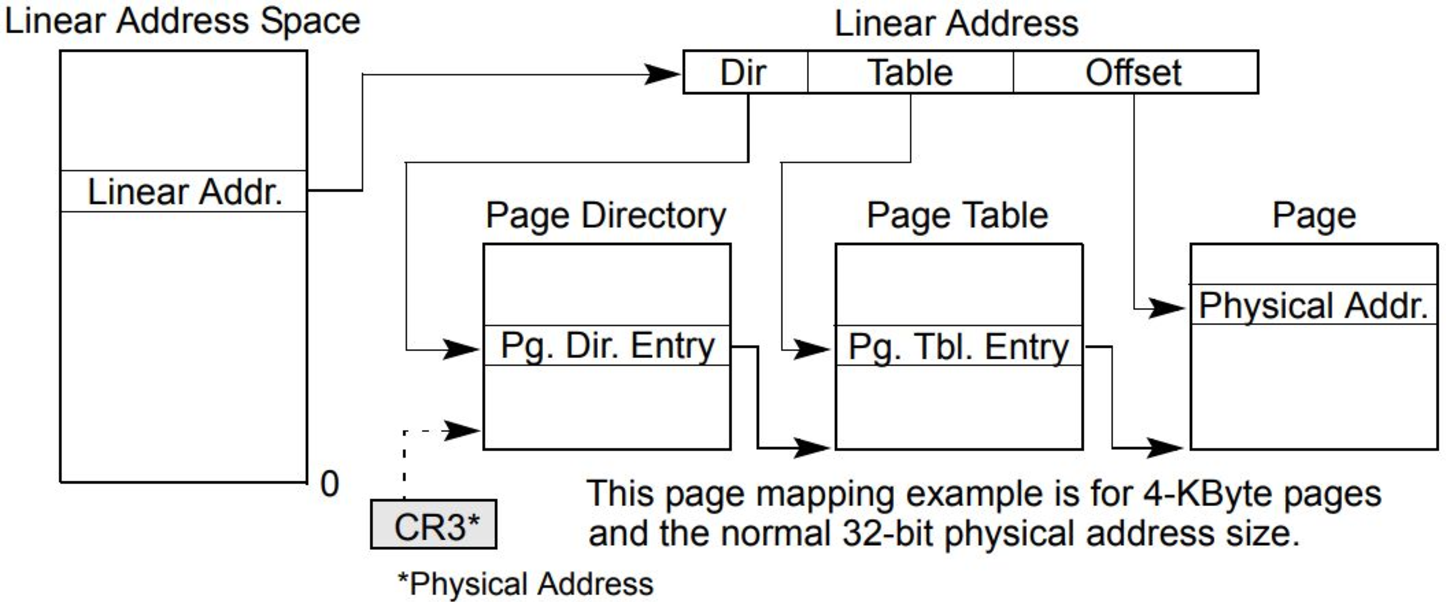
\includegraphics[width=0.47\textwidth]{figures/pagetable}
  \centering
  \caption{Linear-Address Translation to a 4-KBbyte Page using 32-Bit Paging~\cite{guide2011intel}}
  \label{fig:pagetable}
\end{figure}

Every page in the virtual memory has an entry in the page table. As shown in~\autoref{fig:pte}, the \texttt{User/Supervisor} decides whether this is a kernel page or a user page. When set, it is a user page; otherwise, it is a kernel page.

\begin{figure}[th]
  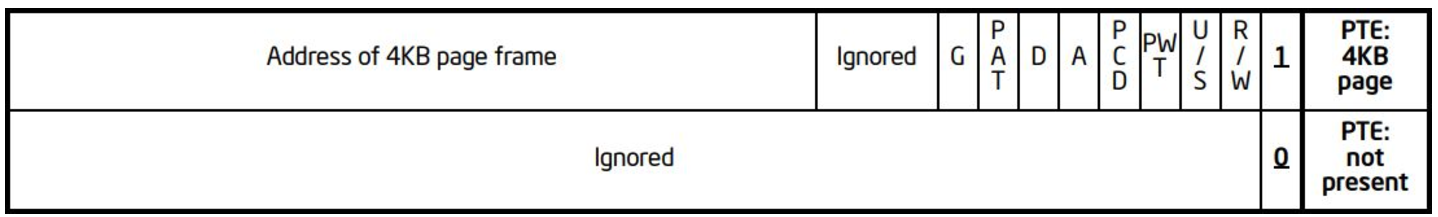
\includegraphics[width=0.47\textwidth]{figures/pte2}
  \centering
  \caption{U/S, the 'User/Supervisor' bit, controls access to the page based on privilege level. If the bit is set, then this page is considered in user mode space and be accessed by all code; if the bit is not set, then it's considered in kernel mode space and can be accessed only by kernel mode code. }
  \label{fig:pte}
\end{figure}



We get various information in the context of a page fault handler. The \texttt{CR2} register stores the faulting virtual address, which, regarding \texttt{SMAP}, is the user-mode address that the kernel accessed. The \texttt{CR3} register stores the physical address of the current page table base, with which we walk through the page table to locate the corresponded \texttt{PTE}. Additionally, we get the error code, \texttt{CS:EIP}, \texttt{SS:ESP} and \texttt{EFLAGS} from the  current kernel stack. Regarding \texttt{SMAP} exception, those are the context frame when the kernel raised the exception. Error code indicates the cause of the exception. We will discuss more details in~\autoref{sec:implementation}.



By changing the \texttt{U/S} bit in a page's \texttt{PTE}, we can change a user-mode page to kernel-mode. On Windows 32-bit system, we usually have the impression that the virtual address above 0x80000000 to 0xFFFFFFFF is the kernel space. However, the system's current privilege level depends on the \texttt{Current Privilege Level (CPL)} field in the \texttt{cs} segment, which is maintained by the CPU. This 2-bit \texttt{CPL} field in the code segment register is always equal to the CPU's current privilege level. In the meantime, the \texttt{U/S} bit in the \texttt{PTE} decides the code of what privilege can access it, and we consider the memory space that only the most privileged code (\texttt{CPL:00}) can run is the kernel space. Indeed, it is a considerably complicated mechanism involving more data structure in the CPU's microarchitecture, out of this paper's scope. In essence, as aforementioned, this bit decides whether the page is a kernel page or a user page, even the virtual address is below 0x80000000 and surrounded by other user pages, as shown in~\autoref{fig:denyuserwrite}.

\begin{figure}[th]
  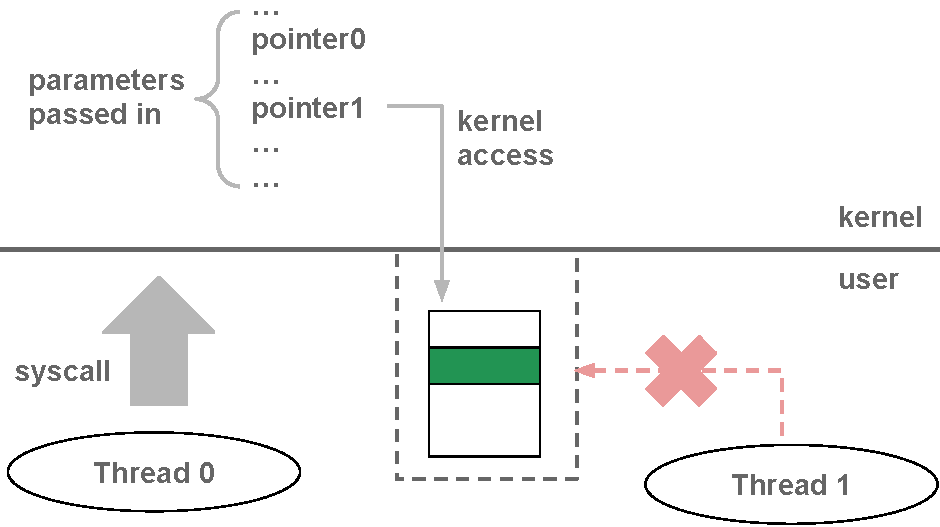
\includegraphics[width=0.37\textwidth]{figures/denyuserwrite}
  \centering
  \caption{User-mode thread 0 initiates a system call with parameters. The system call, which runs in the kernel, access the user-mode memory to get the value. This action raises a SMAP exception and entry the exception handler, within which our mitigation changes the page from user-mode to kernel-mode. Therefore it blocks subsequent accesses from other user-mode threads.}
  \label{fig:denyuserwrite}
\end{figure}




\textbf{\textit{Solving Read Conflicts.}} For practical purposes, solving read conflicts is essential. It is common to have multiple global variables reside on, or multiple heap buffers share the same page. Therefore, when we protect a 4KB page for the kernel, we block benign access to other data.  It is unnecessary because reading does not harm.  

We solve the read conflict by taking the protected page back to userspace. Additionally, in the \texttt{PTE}, we also set \texttt{R/W} bit so that the page is read-only. ~\autoref{fig:pagestate} shows the transitions. It is possible because when other user-mode threads read the protected page, it raises a page fault exception regarding privilege violation due to our protection. Therefore we can handle it and let the thread read the page safely. We also record the original page information to handle various situations and correctly restore it at the end of the system call. 

\begin{figure}[th]
  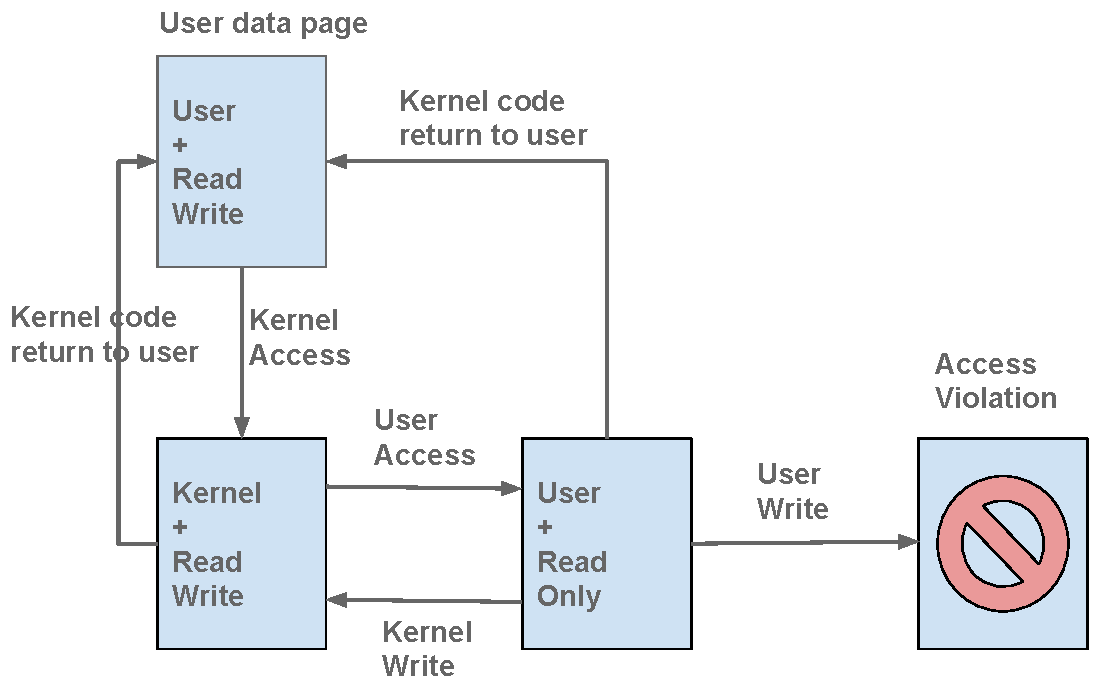
\includegraphics[width=0.30\textwidth]{figures/pagestate}
  \centering
  \caption{Page attributes transit between kernel mode and user mode. When kernel mode code ends, for example, system service returns to user mode, the page will be set back to the original permission}
  \label{fig:pagestate}
\end{figure}




\textbf{\textit{Solving Write Conflicts.}} Unlike the read conflicts, we can not make the page writable at any time. Even the write on the rest of the data is benign. Subject to the x86 architecture, the protection has to base on page granularity. We have to make sure that no user-mode threads write the entire page during the system call. However, we can make them wait then write it after the system call. More specifically, once the write raises an exception, we suspend the thread until the current system call ends. We will discuss why it is possible to suspend a thread inside the page fault handler shortly after.


\begin{figure}[th]
  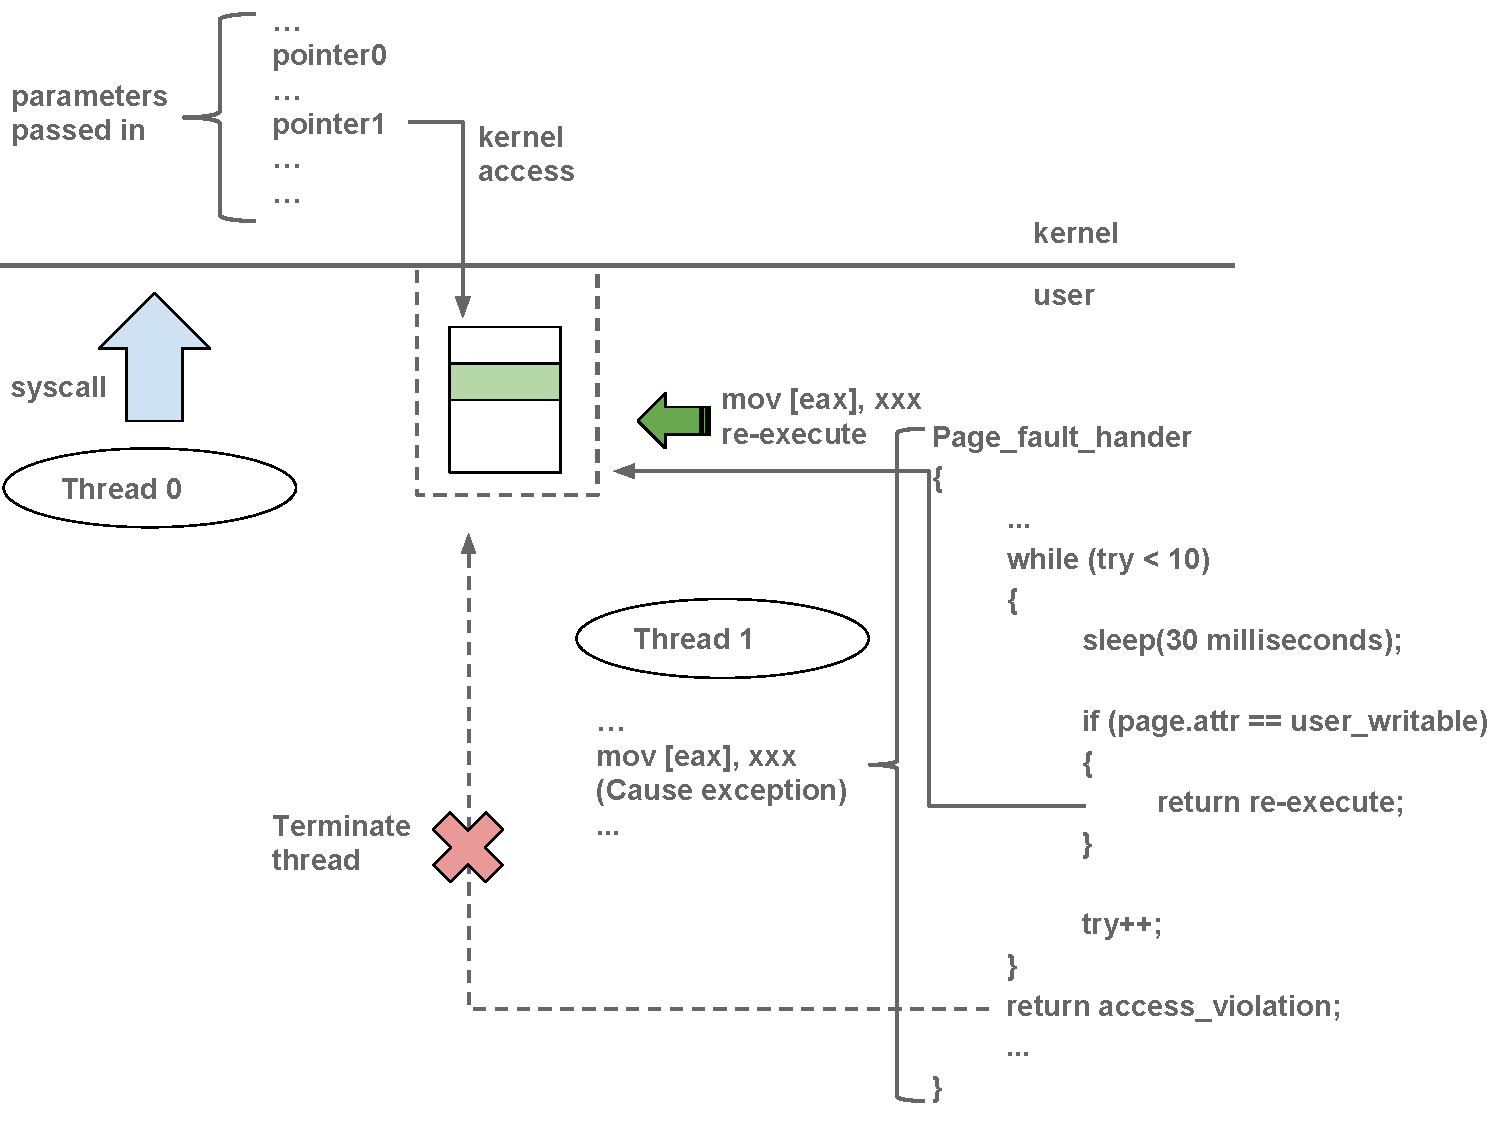
\includegraphics[width=0.47\textwidth]{figures/reexecute}
  \centering
  \caption{We take the delayed access solution when handling a write conflict. Thread one sleeps for a short time in the exception handler, letting the operating system schedule. Recheck the current status when it wakes up. Reexecute the faulting instruction if the protected page is released. Otherwise, wait for the next turn. Moreover, to avoid endless waiting, which may cause a deadlock, the thread will be terminated if it reaches the time threshold.}
  \label{fig:reexecute}
\end{figure}


As shown in ~\autoref{fig:reexecute}, thread 0 invokes a system call with parameters.  \name protects the corresponded page into kernel space once the kernel fetches those parameters. Afterward, thread 1 writes the page, which raises another page fault exception. Inside the handler, \name calls a kernel function, \texttt{KeDelayExecutionTread()}, that suspend the current thread. The thread wakes up periodically to check the page's status. If the page is released, it finishes the exception, re-executes the faulting instruction. Otherwise, \name terminates the thread to prevent any deadlock.

%\subsection{The Differences Between Interrupt and Exception}



\textbf{\textit{Interrupt and Exception.}} Thread suspending inside the page fault handler seems unusual because both interrupts and exceptions have their handler entries in the \texttt{Interrupt Descriptor Table (IDT)}. However, the difference between them is essential.  An interrupt is an asynchronous event that is typically triggered by an I/O device. An exception is a synchronous event generated when the processor detects one or more predefined conditions while executing an instruction. Interrupts have a higher priority than the operating system's scheduler and most of the kernel components. Any job should not take too long inside the interrupt handler~\cite{msdnwatchdog}.  On the contrary, exceptions have the lowest priority in the kernel. In Windows' term, the \texttt{ Interrupt Request Level (IRQL)} that the exception handler executes at is \texttt{PASSIVE\_LEVEL}. It means to call for thread scheduling is plausible.


%\subsection{Releasing Protected Pages}

%Whenever a syscall ends, all the protected page that related to it should be released. Their original attributes will be restored. The Thread Environment Block(TEB) is used to identify each thread within the current process. Each thread has its own TEB data and it's address is easy to locate by segment register FS. 

%We hook a Windows internal function in order to know when it's the end of the syscall. 

%\begin{comment}
%\begin{figure}[th]
%  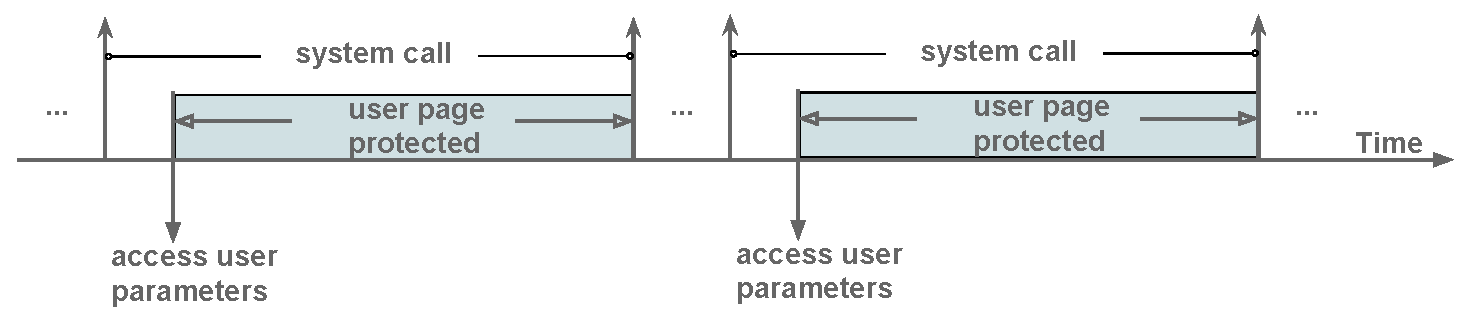
\includegraphics[width=0.40\textwidth]{figures/timeline}
%  \centering
%  \caption{The page protection period is within one system call cycle, this is based on the fact that kernel TOCTOU vulnerability does not happen across system calls.}
%  \label{fig:timeline}
%\end{figure}
%\end{comment}

\textbf{\textit{Releasing Protected Pages.}} To aware when a system call ends, we choose to intercept a Windows internal function. We keep tracking the page table base and \texttt{Thread Environment Block (TEB)} to distinguish each thread so that we release the involved pages on the system call basis.  


%\subsection{TLB Caching}

\textbf{\textit{Flushing TLB.}} To make \texttt{PTE} modifications taking effect on all the processors, we need to flush \texttt{Translation Lookaside Buffer (TLB)}. \texttt{TLB} is a memory cache used to reduce the time taken to access a virtual memory location. It stores the recent translations of virtual memory to physical memory. Different than data cache, TLB is not entirely transparent to the operating system. When the operating system updates a page table entry, the corresponding TLB entry needs to be invalidated.  

As mentioned above, we leverage the page attribute transition to protect and solve conflicts. They are all based on the \texttt{PTE} modification. Hence it is critical to ensure the change on \texttt{PTE} takes effects instantly, especially on a multi-processor system. We examine the method to flush the \texttt{TLB} on the multi-process system through programming the local \texttt{Advanced Programmable Interrupt Controller (APIC)}. Eventually, we find a Windows internal function that flushes \texttt{TLB} entries on all the processors with some reverse-engineering effort. Therefore we do not have to consider the underlying hardware differences.



\subsection{Hypervisor}


For \name, the hypervisor plays an essential role in developing and debugging. When we initially enabled \texttt{SMAP} in Windows, instantly, an enormous amount of exceptions flooded the system. The debugger was frozen.  We expected that because we know Windows does not support this feature, and \texttt{SMAP} is system-wide. Moreover, a significant portion of the system calls fetches user-provided parameters and important system data structures such as \texttt{Process Environment Block (PEB)}, \texttt{USER\_SHARED\_DATA} that mapped in userspace. 

By monitoring the process context switch event, namely, operations on the \texttt{CR3} register, the hypervisor can temporarily enable/disable the \texttt{SMAP} feature to make it only active on a specific process. That is when this process is running on the CPU.

Due to Intel VT virtualization technology's design~\cite{neiger2006intel}, it is possible to load a light-weight hypervisor as a kernel module during run time. Unlike other commercial hypervisors such as Xen, Hyper-V, and VMWare, it does not emulate hardware devices. It merely put the operating system into VM guest mode, and itself becomes the hypervisor, hence monitors system events~\cite{howtohide}.


\begin{figure}[th]
  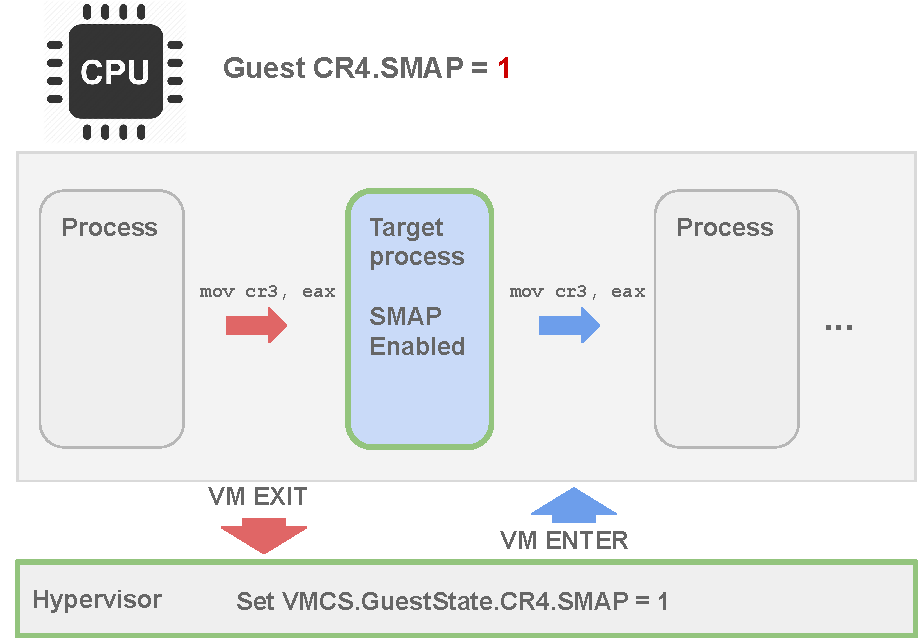
\includegraphics[width=0.40\textwidth]{figures/processmap3}
  \centering
  \caption{Operations on the CR3 register are the decisive characteristic of process context switching, which triggers VM exit by default. By setting the SMAP bit in the CR4 image of the VMCS.GuestArea, it updates the CPU CR4 when the hypervisor enters the virtual machine again. Therefore, it is possible to use the hypervisor to enable the SMAP feature when a specific process is running on the CPU.}
  \label{fig:processmap}
\end{figure}


As shown in~\autoref{fig:processmap}, \texttt{mov cr3, eax} triggers a \texttt{VM Exit} event, and the hypervisor receives it. If the new \texttt{CR3} is one of the target processes, the hypervisor sets the \texttt{CR4.SMAP} in the \texttt{Virtual Machine Control Structure (VMCS)} of the guest virtual machine. It is the data structure that updates the real CPU registers when entering the virtual machine. Back to the guest, the \texttt{SMAP} is active while the process is running. When this process is switching out, the hypervisor again receives the event regarding \texttt{CR3} operation. It then unset \texttt{CR4.SMAP}. Therefore, this particular process will have the illusion that \texttt{SMAP} is active continually while others feel the opposite.

The hypervisor inevitably brings performance overhead. However, it makes the mitigation more configurable. Due to the nature of local privilege escalation attacks, system processes already with high privilege are not likely threats. Hence no protection on them, which reduces the overall overhead.  Additionally, as previously mentioned, to prevent \texttt{SMAP} recurring cased dead loop, the feature isolation is also necessary. Therefore we consider the hypervisor framework as one contribution of this paper.
